\documentclass[12pt, english]{scrartcl} %Koma-Klasse "Artikel" mit 12pt Schrift
\usepackage[left=20mm, right=20mm, top= 25mm, bottom=25mm]{geometry}  % Seitenrändern
\usepackage{graphicx} %zum Einfügen von Bildern
\usepackage[english]{babel} %englische Silbentrennung
\usepackage{multicol}
\usepackage{graphicx}
\usepackage{caption}
\graphicspath{graphics/}
\usepackage{siunitx}

\sisetup{separate-uncertainty}
\usepackage{braket}

\title{F18/38 Atmospheric Spectroscopy}
\author{Carsten L{\"u}th \and Michael Dorkenwald}
\date{\today}

\begin{document}
\maketitle

\begin{multicols}{2}


\section{Abstract}
In this experiment the trace gases Nitrogendioxid ($NO_2$) and Ozone ($O_3$) are examined with DOASIS (DOAS Intelligent System). These trace gases play an important role for life on earth. Therefore it is important to have a method to determine the concentration in the atmosphere. The used system was developed at the Institut for environmental physics at University Heidelberg and can be used to acquire data from a spectrometer and display it in a graphic user interface for evaluation.
\section{Introduction}
Trace gases make up only a very small proportion (less than 0.04 $\%$ of the air. The volume fraction of ozone in the air is 0.04 $ppmv$ and is mainly placed in the stratosphere. Ozone is a highly efficient absorber of the harmful UV radiation. Nitrogen oxides NO and NO2 (together referred as $NO_x$) play an important role in the formation of the so called "Los Angeles Smog" and and are harmful to humans in excessive quantities (700 ppm after 30 minutes will be lethal). In our experiment we first (i) examine NO2  in a gas in our labatory, second (ii) NO2 and Ozone is explored in the atmosphere with a spectrometer placed outside and last (iii) we evaluate the 
\section{Background}

\subsection{Ozone and Nitrogendioxid}

\subsection{The DOAS Measurement System}

\newpage
\section{Meassurements}
\subsection{Nitrogendioxid gas-cell}
In this part of the experiment we measured the absorption of a $NO_2$ gas-cell in the spectrum of an Hg-lamp. Due to the nature of this measurement we could simplify the problem by using the fact that we have access to $I_0$ by taking a spectrum without the gas cell in the light path and then take a measurement with the gas-cell in the light path to measure $I$. After dark current and offset were corrected for both measurements we used the simplified lambert-beer law to get to equation.
\begin{equation}
\tau = \log(\frac{I_0(\lambda)}{I_0(\lambda)})= \sigma_{NO_2} \cdot \rho \cdot L
\end{equation}
The reference convolution for $NO_2$ was then used to compute the SCD$= \rho \cdot L$. This was then used to compute the density $\rho = (2.81 \pm 0.07 ) \cdot 10^{-7} \frac{\text{mol}}{\text{cm}^3}$ and the mixture ratio $(6.29 \pm 0.39) \cdot 10^3 \text{ppm}$.
\subsection{Sunlight of a recorded daycycle}

\subsection{Sunlight different evaluations angles}

\section{Results}
\subsection{Nitrogendioxid gas-cell}
After dark current and offset were corrected for both measurements we used the simplified lambert-beer law to get to equation.
\begin{equation}
\tau = \log(\frac{I_0(\lambda)}{I_0(\lambda)})= \sigma_{NO_2} \cdot \rho \cdot L
\end{equation}
The reference convolution for $NO_2$ was then used to compute the SCD$= \rho \cdot L$. This was then used to compute the density $\rho = (2.81 \pm 0.07 ) \cdot 10^{-7} \frac{\text{mol}}{\text{cm}^3}$ and the mixture ratio $(6.29 \pm 0.39) \cdot 10^3 \text{ppm}$.


\subsection{Sunlight of a recorded daycycle}
The DOAS least squares fit computes the SCD values for the different daytimes and traces gases, namely ozone and nitrogendioxid. Those values were then plotted and can be seen in figures ...
\begin{figure}
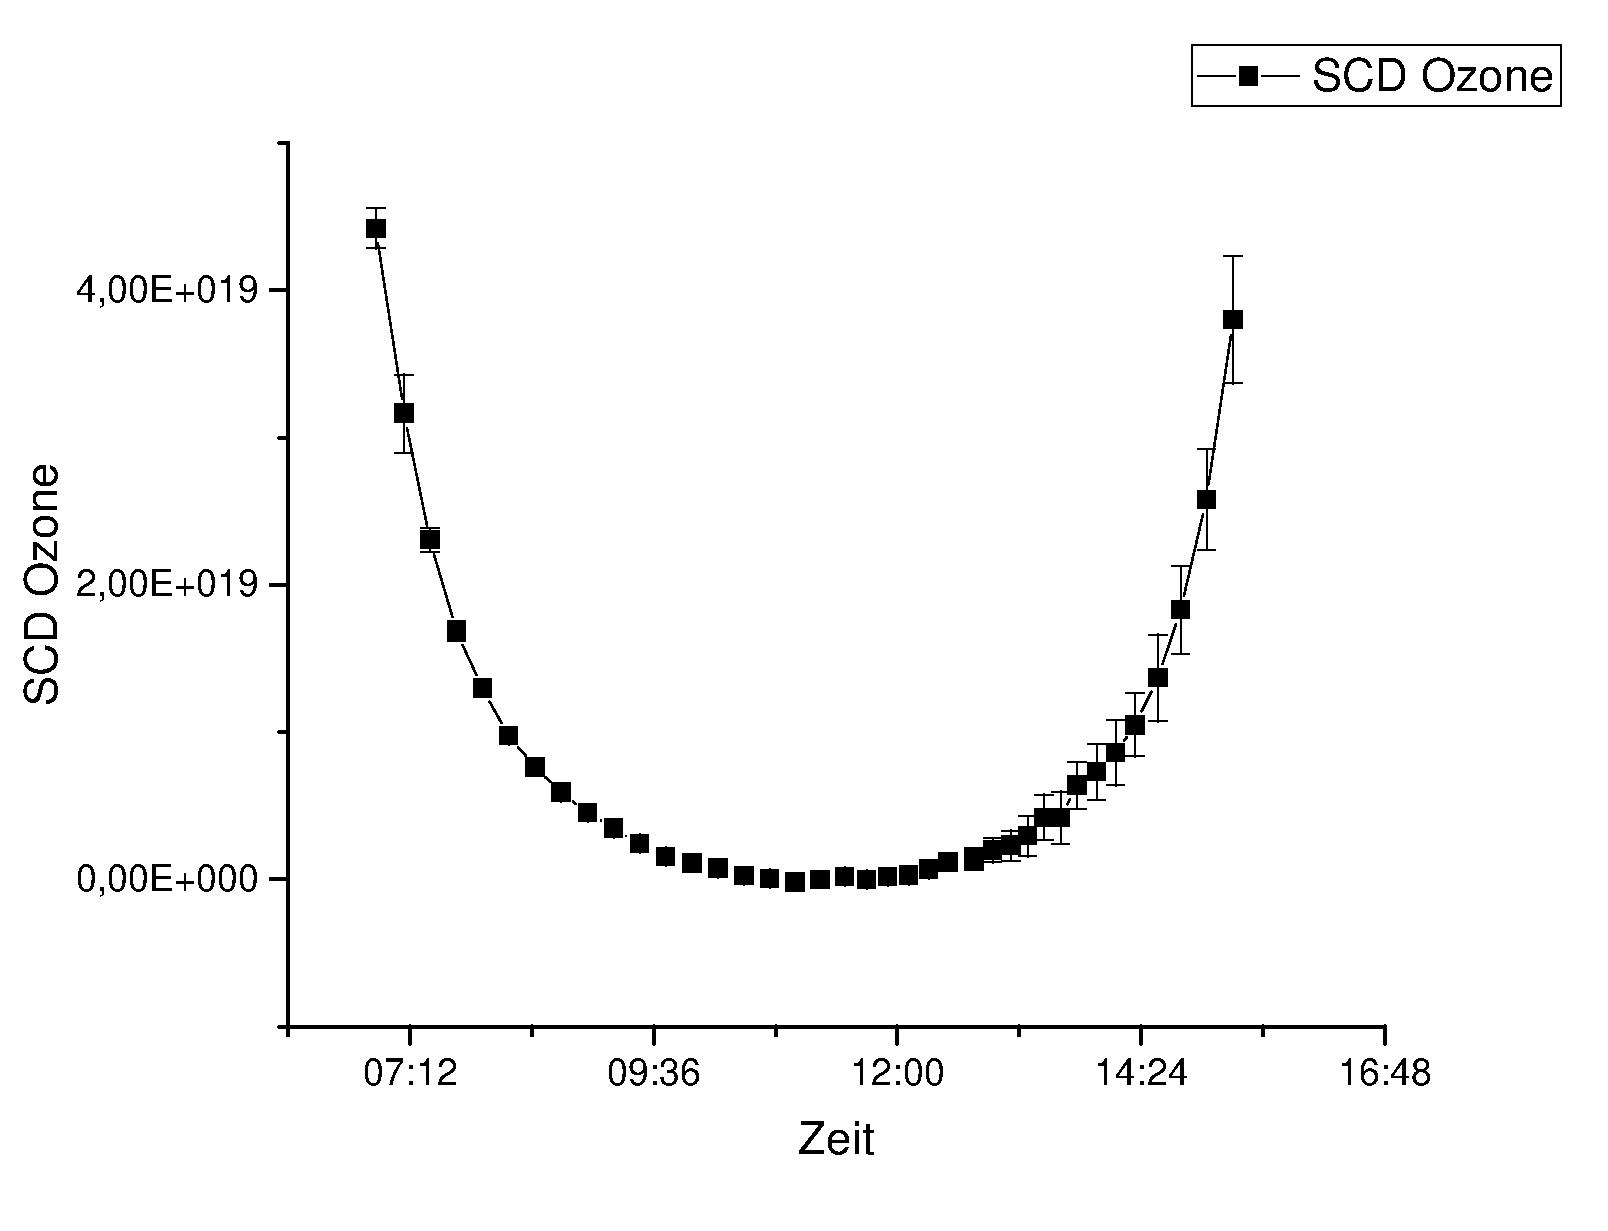
\includegraphics[width= 0.9\textwidth]{graphics/o3scd.pdf}
\end{figure}
asdfasdf

\subsection{Sunlight different evaluations angles}


\section{Discussion}
\end{multicols}

\end{document}